\section{Introduction}
AI hat viele Forschungs- und Anwendungsfälle. In diesem Modul geht es um Algorithmen, also ein Computer lernt von Daten
etwas ähnliches zu machen. $\rightarrow$ \textbf{Statistical Machine Learning}
\\
\textcolor{myblue}{Ziel:} Man programmiert Algorithmus nicht mehr hart, sondern macht ihn lernfähig mit Beispielen. Dies ist wichtiges Merkmal
von Machine Learning und AI.
\\
\textcolor{myblue}{Traum:} Das Entwickeln einer AGI (Artificial general intelligence). Davon sind wir noch weit entfernt und AI können in der Regel
nur ein spezifisches Problem auf mal lösen.
\subsection{Turing Test}
Test, ob AI intelligent ist oder nicht. Testbeschrieb: Person C stellt per Tastatur und Bidschirm eine beliebige Frage an einen anderen Menschen oder KI. Fragesteller weiss nicht wer ihm antwortet. Der Fragesteller entscheidet dann ob es eine Maschine oder der Mensch war. Dazu kann er mehrere Fragen stellen. Die KI ist intelligent, wenn der Mensch diese nicht erkennt.
\\
Dieser Test hat einige Tücken: So muss KI lernen zu lügen und sich dumm zu stellen, da sie ja gleichintelligent wie ein Mensch sein muss.
\subsection{Machine Learning}
Machine Learning ist ein Teilgebiet von AI. Dies wird auch noch weiter unterteilt. Häufig Unterteilung in drei Bereiche:
\textbf{unsupervised}, \textbf{supervised} und \textbf{reinforcement} learning.\\
\textcolor{myblue}{Reinforced Learning:} Hier geht es unter anderem um Spiele: Schachcomputer oder das bekannte GO-Spiel wo AI den Mensch schlägt.
\\
\textcolor{myblue}{Unsupervised Learning:} Hier nimmt man grosse Datenmengen und segmentiert oder clustert diese. Man möchte Daten visualisieren. Beispiel
Politlandschaft.
\\
\textcolor{myblue}{Supervised Learning:} Ein Teil ist die Regression in linearer Algebra. Hier gibt man Daten und Zusatzinformationen (Label). Zum Beispiel gibt man dem Bot Bilder von Hunden und Katzen und lässt ihn lernen diese zu erkennen. Dazu gibt man jeweils auch noch ein Label mit, welches
zeigt welche Bilder von Hunden und welche von Katzen sind.
\section{Dialogflow}
Ein Service von Google, der eine AI im Hintegrund hat für das erstellen von Chatbots: «AI as a Service».
\\
\textcolor{myblue}{Intent:} Kategorisiert Absicht eines Endbenutzers für Unterhaltungsrunde. Im Intent definiert man Trainingssätze, Aktionen und auch
Parameter. So gibt es Dinge die dringend benötigt werden und wenn diese fehlen, müssen diese nachgefragt werden. Weiter kann man unterschiedliche Antworten definieren und der Bot wählt eine zufällig aus.\\
Ein einfacher Intent besteht aus: Training phrases, Actions, Parametern und Responses.\\
Kompliziertere Intents können auch Contexts und Events beinhalten.
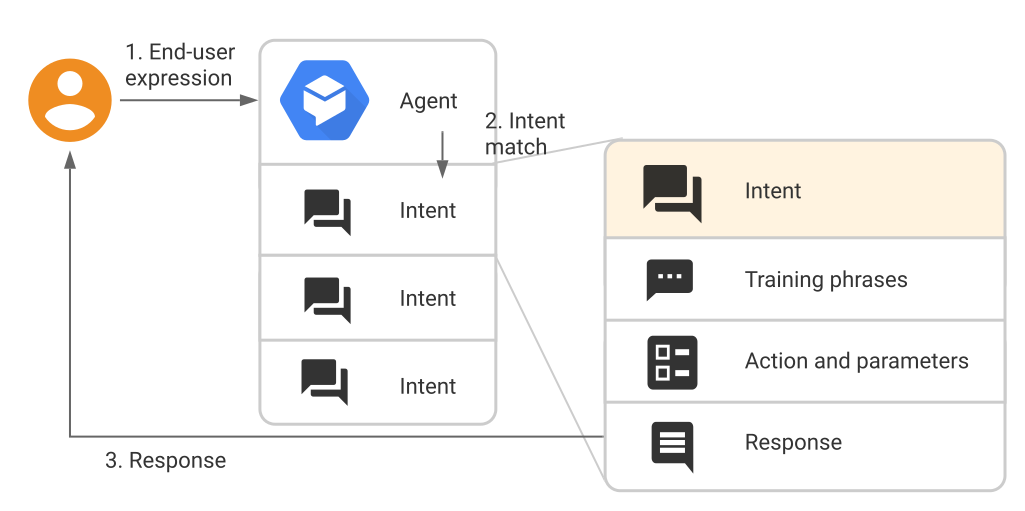
\includegraphics[width=\linewidth]{img/intent-example.png}
\textcolor{myblue}{Entities:} Dienen um einzelne Wörter aus Sätzen auszulesen und zu mappen. Es gibt die Möglichkeit mehrere Trainingsbegriffe zu definieren und auch Synonyme für gleiche Wörter. Auch gibt es die Möglichkeit System-Entities zu verwenden (Vordefinierte Entities, wie Datum und Zeit) \\
\\
Beispiel: What is the \textcolor{blue}{temperature} going to be \textcolor{orange}{tomorrow} in \textcolor{red}{Seattle}?
Durch das Wort \textcolor{blue}{temperature} versteht der Bot, dass ein Forecast gefragt ist (Intent).
\\
Die Wörter \textcolor{orange}{tomorrow} und \textcolor{red}{Seattle} sind Entities für eine Zeit resp einen Ort.
\\
\\
\textcolor{myblue}{Dialog Control (Kontexte):}
Mit Kontexten kann man definieren welcher Intent als nächstes aufgerufen werden sollte, wenn man ein Intent abgeschlossen
hat und kann auch Parameter übergeben, die dann im nächsten Intent verfügbar sind:
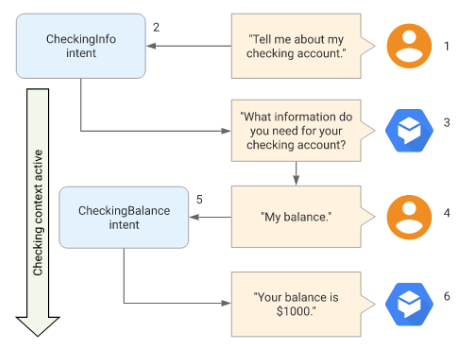
\includegraphics[width=\linewidth]{img/dialog-control.png}